\documentclass[tikz,border=3pt]{standalone}
\usepackage{amsmath,amssymb}
\usetikzlibrary{arrows.meta,calc}

\begin{document}
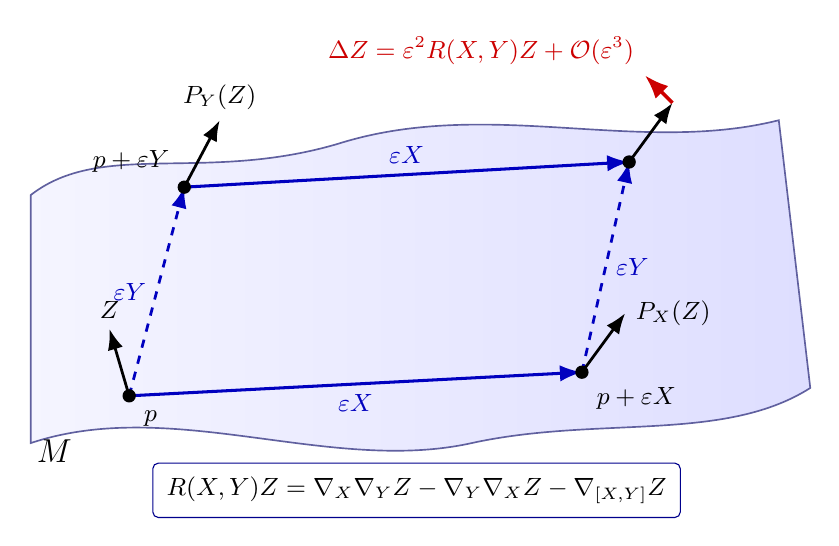
\begin{tikzpicture}[
  >=Latex,
  pathvector/.style={->,line width=1.1pt,blue!75!black},
  transported/.style={->,line width=1pt,dashed,blue!75!black},
  fibre/.style={->,line width=1pt,black},
  point/.style={circle,fill=black,inner sep=1.7pt},
  every node/.style={font=\small}
]
  \path[shade,left color=blue!4,right color=blue!13,draw=blue!25!gray,line width=.6pt]
    (0.2,0.75) .. controls (2.0,1.35) and (4.0,0.35) .. (5.8,0.75)
    .. controls (7.4,1.1) and (9.0,0.75) .. (10.1,1.45)
    -- (9.7,4.85)
    .. controls (7.9,4.4) and (6.0,5.15) .. (4.1,4.55)
    .. controls (2.4,4.05) and (1.1,4.6) .. (0.2,3.9) -- cycle;

  \coordinate (p) at (1.45,1.35);
  \coordinate (px) at (7.2,1.65);
  \coordinate (py) at (2.15,4.0);
  \coordinate (q) at (7.8,4.32);

  \draw[pathvector] (p) -- node[below] {$\varepsilon X$} (px);
  \draw[transported] (px) -- node[right] {$\varepsilon Y$} (q);
  \draw[transported] (p) -- node[left] {$\varepsilon Y$} (py);
  \draw[pathvector] (py) -- node[above] {$\varepsilon X$} (q);

  \draw[fibre] (p) -- ++(-0.25,0.85) node[above] {$Z$};
  \draw[fibre] (px) -- ++(0.55,0.75) node[right] {$P_X(Z)$};
  \draw[fibre] (py) -- ++(0.45,0.85) node[above] {$P_Y(Z)$};
  \draw[fibre] (q) -- ++(0.55,0.75) coordinate (zxy);
  \draw[->,line width=1.25pt,red!80!black] (zxy) -- ++(-0.35,0.35)
    node[above left] {$\Delta Z=\varepsilon^2R(X,Y)Z+\mathcal O(\varepsilon^3)$};

  \node[point,label=below right:{$p$}] at (p) {};
  \node[point,label=below right:{$p+\varepsilon X$}] at (px) {};
  \node[point,label=above left:{$p+\varepsilon Y$}] at (py) {};
  \node[point] at (q) {};
  \node[font=\large] at (0.5,0.65) {$M$};

  \node[draw=blue!55!black,rounded corners=2pt,fill=white,inner sep=5pt]
    at (5.1,0.15) {$R(X,Y)Z=\nabla_X\nabla_YZ-\nabla_Y\nabla_XZ-\nabla_{[X,Y]}Z$};
\end{tikzpicture}
\end{document}
